\documentclass{beamer}
\usetheme{tokitex}

\usepackage{tikz}
\usepackage{graphics}
\usepackage{multirow}
\usepackage{tabto}
\usepackage{xspace}
\usepackage{amsmath}
\usepackage{hyperref}
\usepackage{wrapfig}
\usepackage{mathtools}

\usepackage{tikz}
\usepackage{clrscode3e}
\usepackage{gensymb}

\usepackage[english,bahasa]{babel}
\newtranslation[to=bahasa]{Section}{Bagian}
\newtranslation[to=bahasa]{Subsection}{Subbagian}

\usepackage{listings, lstautogobble}
\usepackage{color}

\definecolor{dkgreen}{rgb}{0,0.6,0}
\definecolor{gray}{rgb}{0.5,0.5,0.5}
\definecolor{mauve}{rgb}{0.58,0,0.82}

\lstset{frame=tb,
  language=c++,
  aboveskip=0mm,
  belowskip=0mm,
  showstringspaces=false,
  columns=fullflexible,
  keepspaces=true,
  basicstyle={\small\ttfamily},
  numbers=none,
  numberstyle=\tiny\color{gray},
  keywordstyle=\color{blue},
  commentstyle=\color{dkgreen},
  stringstyle=\color{mauve},
  breaklines=true,
  breakatwhitespace=true,
  lineskip={-3pt}
}

\usepackage{caption}
\captionsetup[figure]{labelformat=empty}

\newcommand{\progTerm}[1]{\textbf{#1}}
\newcommand{\foreignTerm}[1]{\textit{#1}}
\newcommand{\newTerm}[1]{\alert{\textbf{#1}}}
\newcommand{\emp}[1]{\alert{#1}}
\newcommand{\statement}[1]{"#1"}

\newcommand{\floor}[1]{\lfloor #1 \rfloor}
\newcommand{\ceil}[1]{\lceil #1 \rceil}
\newcommand{\abs}[1]{\left\lvert#1\right\rvert}
\newcommand{\norm}[1]{\left\lVert#1\right\rVert}

% Getting tired of writing \foreignTerm all the time
\newcommand{\farray}{\foreignTerm{array}\xspace}
\newcommand{\fArray}{\foreignTerm{Array}\xspace}
\newcommand{\foverhead}{\foreignTerm{overhead}\xspace}
\newcommand{\fOverhead}{\foreignTerm{Overhead}\xspace}
\newcommand{\fsubarray}{\foreignTerm{subarray}\xspace}
\newcommand{\fSubarray}{\foreignTerm{Subarray}\xspace}
\newcommand{\fbasecase}{\foreignTerm{base case}\xspace}
\newcommand{\fBasecase}{\foreignTerm{Base case}\xspace}
\newcommand{\ftopdown}{\foreignTerm{top-down}\xspace}
\newcommand{\fTopdown}{\foreignTerm{Top-down}\xspace}
\newcommand{\fbottomup}{\foreignTerm{bottom-up}\xspace}
\newcommand{\fBottomup}{\foreignTerm{Bottom-up}\xspace}
\newcommand{\fpruning}{\foreignTerm{pruning}\xspace}
\newcommand{\fPruning}{\foreignTerm{Pruning}\xspace}

\newcommand{\fgraph}{\foreignTerm{graph}\xspace}
\newcommand{\fGraph}{\foreignTerm{Graph}\xspace}
\newcommand{\froot}{\foreignTerm{root}\xspace}
\newcommand{\fRoot}{\foreignTerm{Root}\xspace}
\newcommand{\fnode}{\foreignTerm{node}\xspace}
\newcommand{\fNode}{\foreignTerm{Node}\xspace}
\newcommand{\fedge}{\foreignTerm{edge}\xspace}
\newcommand{\fEdge}{\foreignTerm{Edge}\xspace}
\newcommand{\fcycle}{\foreignTerm{cycle}\xspace}
\newcommand{\fCycle}{\foreignTerm{Cycle}\xspace}
\newcommand{\fdegree}{\foreignTerm{degree}\xspace}
\newcommand{\fDegree}{\foreignTerm{Degree}\xspace}
\newcommand{\fadjacencylist}{\foreignTerm{adjacency list}\xspace}
\newcommand{\fAdjacencylist}{\foreignTerm{Adjacency list}\xspace}
\newcommand{\fadjacencymatrix}{\foreignTerm{adjacency matrix}\xspace}
\newcommand{\fAdjacencymatrix}{\foreignTerm{Adjacency matrix}\xspace}
\newcommand{\fedgelist}{\foreignTerm{edge list}\xspace}
\newcommand{\fEdgelist}{\foreignTerm{Edge list}\xspace}
\newcommand{\flist}{\foreignTerm{list}\xspace}
\newcommand{\fList}{\foreignTerm{List}\xspace}
\newcommand{\fgraphtraversal}{\foreignTerm{graph traversal}\xspace}
\newcommand{\fGraphtraversal}{\foreignTerm{Graph traversal}\xspace}
\newcommand{\ftree}{\foreignTerm{tree}\xspace}
\newcommand{\fTree}{\foreignTerm{Tree}\xspace}
\newcommand{\fsubtree}{\foreignTerm{subtree}\xspace}
\newcommand{\fSubtree}{\foreignTerm{Subtree}\xspace}
\newcommand{\fparent}{\foreignTerm{parent}\xspace}
\newcommand{\fParent}{\foreignTerm{Parent}\xspace}
\newcommand{\fsibling}{\foreignTerm{sibling}\xspace}
\newcommand{\fSibling}{\foreignTerm{Sibling}\xspace}
\newcommand{\fpath}{\foreignTerm{path}\xspace}
\newcommand{\fPath}{\foreignTerm{Path}\xspace}
\newcommand{\fconnectedcomponent}{\foreignTerm{connected component}\xspace}
\newcommand{\fConnectedcomponent}{\foreignTerm{Connected component}\xspace}
\newcommand{\fbridge}{\foreignTerm{bridge}\xspace}
\newcommand{\fBridge}{\foreignTerm{Bridge}\xspace}
\newcommand{\farticulationpoint}{\foreignTerm{articulation point}\xspace}
\newcommand{\fArticulationpoint}{\foreignTerm{Articulation point}\xspace}
\newcommand{\ftreeedge}{\foreignTerm{tree edge}\xspace}
\newcommand{\fTreeedge}{\foreignTerm{Tree edge}\xspace}
\newcommand{\fbackedge}{\foreignTerm{back edge}\xspace}
\newcommand{\fBackedge}{\foreignTerm{Back edge}\xspace}
\newcommand{\fforwardedge}{\foreignTerm{forward edge}\xspace}
\newcommand{\fForwardedge}{\foreignTerm{Forward edge}\xspace}
\newcommand{\fcrossedge}{\foreignTerm{cross edge}\xspace}
\newcommand{\fCrossedge}{\foreignTerm{Cross edge}\xspace}
\newcommand{\fdiscoverytime}{\foreignTerm{discovery time}\xspace}
\newcommand{\fDiscoverytime}{\foreignTerm{Discovery time}\xspace}
\newcommand{\flowlink}{\foreignTerm{low link}\xspace}
\newcommand{\fLowlink}{\foreignTerm{Low link}\xspace}
\newcommand{\fstack}{\foreignTerm{stack}\xspace}
\newcommand{\fStack}{\foreignTerm{Stack}\xspace}
\newcommand{\for}{\foreignTerm{or}\xspace}
\newcommand{\fOr}{\foreignTerm{Or}\xspace}
\newcommand{\fand}{\foreignTerm{and}\xspace}
\newcommand{\fAnd}{\foreignTerm{And}\xspace}
\newcommand{\fcentroid}{\foreignTerm{centroid}\xspace}
\newcommand{\fCentroid}{\foreignTerm{Centroid}\xspace}

\newcommand{\fDivideAndConquer}{\foreignTerm{Divide and conquer}\xspace}
\newcommand{\fdivideAndConquer}{\foreignTerm{divide and conquer}\xspace}
\newcommand{\fMergeSort}{\foreignTerm{Merge sort}\xspace}
\newcommand{\fmergeSort}{\foreignTerm{merge sort}\xspace}
\newcommand{\fQuickSort}{\foreignTerm{Quicksort}\xspace}
\newcommand{\fquickSort}{\foreignTerm{quicksort}\xspace}
\newcommand{\fpivot}{\foreignTerm{pivot}\xspace}
\newcommand{\fPivot}{\foreignTerm{Pivot}\xspace}
\newcommand{\fbruteForce}{\foreignTerm{brute force}\xspace}
\newcommand{\fBruteForce}{\foreignTerm{Brute force}\xspace}
\newcommand{\fCompleteSearch}{\foreignTerm{complete search}\xspace}
\newcommand{\fExhaustiveSearch}{\foreignTerm{exhaustive search}\xspace}
\newcommand{\fbinarySearch}{\foreignTerm{binary search}\xspace}
\newcommand{\fBinarySearch}{\foreignTerm{Binary search}\xspace}
\newcommand{\fternarySearch}{\foreignTerm{ternary search}\xspace}
\newcommand{\fTernarySearch}{\foreignTerm{Ternary search}\xspace}
\newcommand{\funimodal}{\foreignTerm{unimodal}\xspace}
\newcommand{\fUnimodal}{\foreignTerm{Unimodal}\xspace}
\newcommand{\fGreedy}{\foreignTerm{Greedy}\xspace}
\newcommand{\fgreedy}{\foreignTerm{greedy}\xspace}
\newcommand{\fgreedyChoice}{\foreignTerm{greedy choice}\xspace}
\newcommand{\fGreedyChoice}{\foreignTerm{Greedy choice}\xspace}

\newcommand{\fdp}{\foreignTerm{dynamic programming}\xspace}
\newcommand{\fDp}{\foreignTerm{Dynamic programming}\xspace}
\newcommand{\fbitmask}{\foreignTerm{bitmask}\xspace}
\newcommand{\fBitmask}{\foreignTerm{Bitmask}\xspace}
\newcommand{\fstate}{\foreignTerm{state}\xspace}
\newcommand{\fState}{\foreignTerm{State}\xspace}
\newcommand{\fsubmask}{\foreignTerm{submask}\xspace}
\newcommand{\fSubmask}{\foreignTerm{Submask}\xspace}

\newcommand{\pheap}{\foreignTerm{heap}\xspace}
\newcommand{\pHeap}{\foreignTerm{Heap}\xspace}
\newcommand{\pBinaryHeap}{\foreignTerm{Binary Heap}\xspace}
\newcommand{\pbinaryHeap}{\foreignTerm{binary heap}\xspace}
\newcommand{\pHeapsort}{\foreignTerm{Heapsort}\xspace}
\newcommand{\pheapsort}{\foreignTerm{heapsort}\xspace}
\newcommand{\pdjs}{\foreignTerm{disjoint set}\xspace}
\newcommand{\pDjs}{\foreignTerm{Disjoint set}\xspace}

\newcommand{\fdotProduct}{\foreignTerm{dot product}\xspace}
\newcommand{\fDotProduct}{\foreignTerm{Dot product}\xspace}
\newcommand{\fcrossProduct}{\foreignTerm{cross product}\xspace}
\newcommand{\fCrossProduct}{\foreignTerm{Cross product}\xspace}
\newcommand{\fconvexHull}{\foreignTerm{convex hull}\xspace}
\newcommand{\fConvexHull}{\foreignTerm{Convex hull}\xspace}
\newcommand{\fgrahamScan}{\foreignTerm{graham scan}\xspace}
\newcommand{\fGrahamScan}{\foreignTerm{Graham scan}\xspace}
\newcommand{\flineSweep}{\foreignTerm{line sweep}\xspace}
\newcommand{\fLineSweep}{\foreignTerm{Line sweep}\xspace}

\newcommand{\fset}{\foreignTerm{set}\xspace}
\newcommand{\fSet}{\foreignTerm{Set}\xspace}
\newcommand{\fprefixSum}{\foreignTerm{prefix sum}\xspace}
\newcommand{\fPrefixSum}{\foreignTerm{Prefix sum}\xspace}
\newcommand{\ffenwickTree}{\foreignTerm{fenwick tree}\xspace}
\newcommand{\fFenwickTree}{\foreignTerm{Fenwick tree}\xspace}
\newcommand{\frangeSumQuery}{\foreignTerm{range sum query}\xspace}
\newcommand{\fRangeSumQuery}{\foreignTerm{Range sum query}\xspace}
\newcommand{\fquery}{\foreignTerm{query}\xspace}
\newcommand{\fQuery}{\foreignTerm{Query}\xspace}
\newcommand{\fsegmentTree}{\foreignTerm{segment tree}\xspace}
\newcommand{\fSegmentTree}{\foreignTerm{Segment tree}\xspace}
\newcommand{\fbinaryTree}{\foreignTerm{binary tree}\xspace}
\newcommand{\fBinaryTree}{\foreignTerm{Binary tree}\xspace}
\newcommand{\flazyPropagation}{\foreignTerm{lazy propagation}\xspace}
\newcommand{\fLazyPropagation}{\foreignTerm{Lazy propagation}\xspace}
\newcommand{\fsparseTable}{\foreignTerm{sparse table}\xspace}
\newcommand{\fSparseTable}{\foreignTerm{Sparse table}\xspace}

\newcommand{\ftrail}{\foreignTerm{trail}\xspace}
\newcommand{\fTrail}{\foreignTerm{Trail}\xspace}
\newcommand{\feulerTour}{\foreignTerm{euler tour}\xspace}
\newcommand{\fEulerTour}{\foreignTerm{Euler tour}\xspace}
\newcommand{\feulerTourTree}{\foreignTerm{euler tour tree}\xspace}
\newcommand{\fEulerTourTree}{\foreignTerm{Euler tour tree}\xspace}

\newcommand{\fmaxflow}{\foreignTerm{maximum flow}\xspace}
\newcommand{\fMaxflow}{\foreignTerm{Maximum flow}\xspace}
\newcommand{\fmincut}{\foreignTerm{minimum cut}\xspace}
\newcommand{\fMincut}{\foreignTerm{Minimum cut}\xspace}
\newcommand{\fflow}{\foreignTerm{flow}\xspace}
\newcommand{\fFlow}{\foreignTerm{Flow}\xspace}
\newcommand{\fsource}{\foreignTerm{source}\xspace}
\newcommand{\fSource}{\foreignTerm{Source}\xspace}
\newcommand{\fsink}{\foreignTerm{sink}\xspace}
\newcommand{\fSink}{\foreignTerm{Sink}\xspace}
\newcommand{\fbackEdge}{\foreignTerm{back-edge}\xspace}
\newcommand{\fBackEdge}{\foreignTerm{Back-edge}\xspace}
\newcommand{\fresidualCapacity}{\foreignTerm{residual capacity}\xspace}
\newcommand{\fResidualCapacity}{\foreignTerm{Residual capacity}\xspace}
\newcommand{\fbottleneck}{\foreignTerm{bottleneck}\xspace}
\newcommand{\fBottleneck}{\foreignTerm{Bottleneck}\xspace}
\newcommand{\faugmentingPath}{\foreignTerm{augmenting path}\xspace}
\newcommand{\fAugmentingPath}{\foreignTerm{Augmenting path}\xspace}


\title{Dynamic Programming Lanjutan}
\author{Tim Olimpiade Komputer Indonesia}
\date{}

\begin{document}

\begin{frame}
\titlepage
\end{frame}

\begin{frame}
\frametitle{Pendahuluan}
Melalui dokumen ini, kalian akan:
\begin{itemize}
  \item Memahami konsep \fbitmask
  \item Memahami penggunaan DP menggunakan \fbitmask
  \item Memahami penggunaan DP pada \ftree
\end{itemize}
\end{frame}

\begin{frame}
\frametitle{Motivasi}
\begin{itemize}
  \item Diberikan sebuah struktur kota dan jalan.
  \item Terdapat $V$ kota, dan $E$ ruas jalan.
  \item Setiap ruas jalan memiliki panjang yang berbeda-beda dan menghubungkan dua kota.
  \item Tentukan berapa jarak terpendek untuk mengunjungi seluruh kota tepat sekali.
\end{itemize}
\end{frame}

\begin{frame}
\frametitle{Mengenal Bitmask}
\begin{itemize}
  \item \newTerm{Bitmask} adalah salah satu cara merepresentasikan subhimpunan dari himpunan $\{0, 1, 2, ..., N - 1\}$ dengan menggunakan bilangan bulat dari $0$ sampai $2^N - 1$.
  \item Bilangan $i$ berada pada subhimpunan jika dan hanya jika bit ke-$i$ pada representasi biner pada bilangan representasi subhimpunannya adalah $1$.
  \begin{itemize}
    \item Dengan kata lain, jika bilangan $i$ berada pada subhimpunan, maka tambahkan $2^i$ pada bilangan representasinya.
  \end{itemize}
  \item Sebagai contoh, subhimpunan $\{0, 3, 4\}$ dapat direpresentasikan dengan 25 dan subhimpunan $\{\}$ dapat direpresentasikan dengan $0$.
\end{itemize}
\end{frame}

\begin{frame}
\frametitle{Operasi Bitmask}
\begin{itemize}
  \item Terdapat beberapa operasi dua \fbitmask. Jika $x$ dan $y$ adalah dua \fbitmask.
  \begin{itemize}
    \item $x \text{ or } y$ akan mengembalikan \fbitmask yang merupakan \fbitmask yang merepresentasikan gabungan dari himpunan yang direpresentasikan oleh $x$ dan $y$.
    \begin{itemize}
      \item Sebagai contoh, $25 \text{ or } 3 = 27$ karena gabungan dari $\{0, 3, 4\}$ dan $\{0, 1\}$ adalah $\{0, 1, 3, 4\}$.
      \item Pada C++, operasi ini dihitung dengan \lstinline{x | y}.
    \end{itemize}
    \item $x \text{ and } y$ akan mengembalikan \fbitmask yang merupakan \fbitmask yang merepresentasikan irisan dari himpunan yang direpresentasikan oleh $x$ dan $y$.
    \begin{itemize}
      \item Sebagai contoh, $25 \text{ and } 3 = 1$ karena irisan dari $\{0, 3, 4\}$ dan $\{0, 1\}$ adalah $\{0\}$.
      \item Pada C++, operasi ini dihitung dengan \lstinline{x & y}.
    \end{itemize}
  \end{itemize}
\end{itemize}
\end{frame}

\begin{frame}
\frametitle{Operasi Bitmask (lanj.)}
\begin{itemize}
  \item Dengan operasi tersebut, kita dapat memeriksa beberapa properti sebuah \fbitmask dengan mudah.
  \begin{itemize}
    \item Memeriksa apakah subhimpunan yang direpresentasikan oleh \fbitmask $x$ berisi bilangan $i$ dapat dilakukan dengan memeriksa apakah irisan subhimpunan tersebut dan $\{i\}$ merupakan himpunan kosong.
    \begin{itemize}
      \item \lstinline{(x & (1 << i)) > 0  // `true' jika subhimpunan berisi i.}
    \end{itemize}
    \item Memeriksa apakah subhimpunan berisi seluruh bilangan dari $0$ sampai $N - 1$.
    \begin{itemize}
      \item \lstinline{x == ((1 << N) - 1)  // `true' jika subhimpunan berisi seluruh bilangan dari 0 sampai N - 1.}
    \end{itemize}
  \end{itemize}
\end{itemize}
\end{frame}

\begin{frame}
\frametitle{DP bitmask: Travelling Salesman Problem}
\begin{itemize}
  \item Tentukan berapa jarak terpendek untuk mengunjungi seluruh kota tepat sekali pada sebuah \fgraph. Soal ini merupakan soal klasik yang disebut \newTerm{Travelling Salesman Problem} (TSP).
  \item Hal ini dapat dihitung dengan menggunakan \fdp dengan menyimpan subhimpunan kota yang sudah pernah dikunjungi dan kota yang sekarang sedang dikunjungi sebagai parameter fungsi.
  \item Fungsi dapat dihitung dengan mencoba seluruh kemungkinan kota yang berikutnya ingin dikunjungi.
\end{itemize}
\end{frame}

\begin{frame}[fragile]  
\frametitle{Solusi TSP menggunakan DP Top-Down}
\begin{lstlisting}
int solve(int mask, int u) {
  if (mask == (1 << N) - 1) {
    return 0;  // seluruh kota sudah dikunjungi
  }
  if (computed[mask][u]) {
    return memo[mask][u];
  }
  computed[mask][u] = true;
  int res = INT_MAX;
  for (int v : adj[u]) {
    if ((mask & (1 << v)) == 0) {  // kota v belum dikunjungi
      res = min(res, solve(mask | (1 << v), mask) + length[u][v]);
    }
  }
  return memo[mask][u] = res;
}
\end{lstlisting}
\end{frame}

\begin{frame}
\frametitle{Kompleksitas Solusi TSP}
\begin{itemize}
  \item Jawaban TSP yang diinginkan adalah minimum dari \lstinline{solve(1 << u, u)} untuk seluruh \lstinline{u}.
  \item Banyaknya kemungkinan parameter pada fungsi \lstinline{solve} di slide sebelumnya adalah $O(2^N \times N)$.
  \item Setiap fungsi \lstinline{solve} mencoba seluruh kemungkinan kota yang berikutnya dikunjungi, sehingga membutuhkan waktu $O(N)$.
  \item Sehingga, total kompleksitas dari solusi \fdp ini adalah $O(2^N \times N^2)$.
\end{itemize}
\end{frame}

\begin{frame}
\frametitle{DP Broken Profile: Contoh Soal}
Diberikan grid yang berisi $R \times C$ sel. Setiap sel berisi sebuah bilangan bulat. Anda ingin mengambil beberapa sel sedemikian sehingga total bilangan bulat pada sel yang Anda ambil semaksimum mungkin dan tidak terdapat tiga sel yang diambil bersebelahan dengan bentuk
\newline
\begin{center}
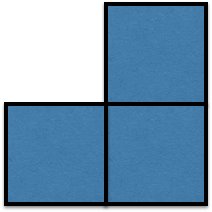
\includegraphics[width=3cm]{asset/shape.png}
\end{center}
\end{frame}

\begin{frame}
\frametitle{DP Broken Profile}
\begin{itemize}
  \item Kita dapat mencoba apakah setiap sel akan diambil atau tidak dengan urutan sel
  \newline
  $(1, 1), (1, 2), \dots, (1, C),$
  \newline
  $(2, 1), (2, 2), \dots, (2, C),$
  \newline
  $\dots$
  \newline
  $(R, 1), (R, 2), \dots, (R, C)$.
  \item Dengan menyimpan apakah $C$ sel terakhir diambil atau tidak dan lokasi sel sekarang, kita dapat mengetahui apakah sel sekarang dapat diambil atau tidak.
  \begin{itemize}
    \item Selain sel pada kolom pertama, jika satu sel sebelumnya (sel di kirinya) dan $C$ sel sebelumnya (sel di atasnya) sudah diambil, maka sel sekarang tidak dapat diambil.
    \item \fState $C$ sel terakhir dapat direpresentasikan menggunakan \fbitmask. Bit ke-$i$ pada \fbitmask merupakan bit $1$ jika dan hanya jika $i$ sel sebelumnya diambil.
  \end{itemize}
\end{itemize}
\end{frame}

\begin{frame}[fragile]
\frametitle{Solusi menggunakan DP Top-Down}
\begin{lstlisting}
int dp(int mask, int now) {
  if (now.r == R + 1) {
    return 0;  // seluruh sel telah diiterasi.
  }
  if (computed[mask][now]) {
    return memo[mask][now];
  }
  computed[mask][now] = true;
  int next_mask = (mask << 1) % (1 << C);
  int res = dp(next(now), next_mask);  // sel sekarang tidak diambil.
  if (now.c == 1 || !(mask & 1) || !(mask & (1 << (C - 1))) {
    // antara sel di kirinya atau sel di atasnya tidak diambil.
    res = max(res, dp(next(now), next_mask + 1) + value[now]);
  }
  return memo[mask][now] = res;
}
\end{lstlisting}
\end{frame}

\begin{frame}
\frametitle{Kompleksitas Solusi}
\begin{itemize}
  \item Jawaban yang diinginkan adalah \lstinline{dp(0, (1, 1))}.
  \item Banyaknya kemungkinan parameter pada fungsi \lstinline{dp} di slide sebelumnya adalah $O(2^C \times R \times C)$.
  \item Setiap fungsi \lstinline{dp} mencoba hanya dua kemungkinan, sehingga membutuhkan waktu $O(1)$.
  \item Sehingga, total kompleksitas dari solusi \fdp ini adalah $O(2^C \times R \times C)$.
\end{itemize}
\end{frame}

\begin{frame}
\frametitle{DP Sum over Subset}
\begin{itemize}
  \item Misalkan ada 2 \fbitmask $x$ dan $y$. $x$ dikatakan \newTerm{submask} dari $y$ jika dan hanya jika $x \text{ and } y = x$. Dengan kata lain, subhimpunan yang direpresentasikan oleh \fbitmask $x$ merupakan subhimpunan dari subhimpunan yang direpresentasikan oleh \fbitmask $y$.
  \item Diberikan sebuah array $F$ berisi $N$ bilangan bulat. Untuk setiap \fbitmask $M (0 \le M < 2^N)$, Anda diminta mencari jumlah $F[X]$ untuk semua $X$ \fsubmask dari $M$.
\end{itemize}
\end{frame}

\begin{frame}
\frametitle{DP Sum over Subset (lanj.)}
\begin{itemize}
  \item Persoalan ini dapat diselesaikan menggunakan DP.
  \item Untuk \fbitmask $M$ dan bilangan bulat $i$, didefinisikan $S(M, i)$ sebagai himpunan \fbitmask $m$ yang merupakan submask $M$ dan hanya $i$ bit pertamanya yang boleh berbeda.
  \begin{itemize}
    \item Bit pertama adalah bit dengan bobot $2^0$, yang ditulis paling kanan pada representasi biner.
    \item Dengan kata lain, $m$ berada pada himpunan $S(M, i)$ jika dan hanya $m$ merupakan submask $M$ dan $M - m < 2^i$.
  \end{itemize}
  \item Sebagai contoh, $S(\textbf{101}01, 2) = \{\textbf{101}00, \textbf{101}11\}$ dan $S(\textbf{10}101, 3) = \{\textbf{10}000, \textbf{10}001, \textbf{10}100, \textbf{10}111\}$.
\end{itemize}
\end{frame}

\begin{frame}
\frametitle{DP Sum over Subset (lanj.)}
\begin{itemize}
  \item Perhatikan bahwa S(M, i) dapat dihitung secara rekursif sebagai berikut:
  \begin{itemize}
    \item $S(M, 0) = \{M\}$
    \item $S(M, i) = S(M, i - 1)$ jika bit ke-$(i - 1)$ pada $M$ adalah $0$.
    \item $S(M, i) = S(M, i - 1) \cup S(M - 2^i - 1, i - 1)$ jika bit ke-$(i - 1)$ pada $M$ adalah $1$. Perhatikan bahwa $S(M, i - 1) \cap S(M - 2^i - 1, i - 1) = \emptyset$
  \end{itemize}
  \item Kita dapat definisikan $DP(M, i)$ sebagai jumlah $F[x]$ untuk setiap $x$ yang merupakan anggota dari $S(M, i)$. Sehingga, $DP(M, i)$ dapat dihitung sebagai beriukt:
  \begin{itemize}
    \item $DP(M, 0) = F[M]$
    \item $DP(M, i) = DP(M, i - 1)$ jika bit ke-$(i - 1)$ pada $M$ adalah $0$.
    \item $DP(M, i) = DP(M, i - 1) + DP(M - 2i - 1, i - 1)$ jika bit ke-$(i - 1)$ pada $M$ adalah $1$.
  \end{itemize}
\end{itemize}
\end{frame}

\begin{frame}
\frametitle{Kompleksitas Solusi}
\begin{itemize}
  \item Jawaban yang diinginkan untuk \fbitmask $F[M]$ adalah $DP(M, N)$.
  \item Banyaknya kemungkinan parameter pada fungsi $DP$ di slide sebelumnya adalah $O(2^N \times N)$.
  \item Setiap fungsi $DP$ mencoba hanya dua kemungkinan, sehingga membutuhkan waktu $O(1)$.
  \item Sehingga, total kompleksitas dari solusi \fdp ini adalah $O(2^N \times N)$.
\end{itemize}
\end{frame}

\begin{frame}
\frametitle{DP pada complete binary tree: Contoh Soal}
\begin{itemize}
  \item Diberikan sebuah \foreignTerm{complete binary tree}\xspace dengan setiap \fnode memiliki bobot.
  \item Anda ingin mengambil $K$ \fnode sedemikian sehingga total bobot dari \fnode yang diambil semaksimum mungkin dan jika sebuah \fnode diambil, maka \fparent dari \fnode tersebut tidak boleh diambil.
\end{itemize}
\end{frame}

\begin{frame}
\frametitle{DP pada complete binary tree}
\begin{itemize}
  \item Persoalan ini dapat diselesaikan dengan mendefinisikan $f(u, root, take)$, dengan $u$ adalah \fnode pada tree, $root$ adalah sebuah boolean, dan $take$ adalah sebuah bilangan bulat, sebagai berikut:
  \begin{itemize}
    \item Kita ingin mengambil $take$ \fnode yang merupakan \fsubtree dari $u$.
    \item \fNode $u$ dapat diambil jika dan hanya jika $root = true$.
    \item Fungsi ini mengembalikan maksimum total bobot \fnode yang dapat diambil.
  \end{itemize}
  \item Fungsi ini dapat dihitung dengan mencoba:
  \begin{itemize}
    \item apakah \fnode $u$ akan diambil,
    \item ada berapa \fnode yang ingin diambil yang merupakan \fsubtree dari anak $u$ pertama, dan
    \item ada berapa \fnode yang ingin diambil yang merupakan \fsubtree dari anak $u$ kedua.
  \end{itemize}
\end{itemize}
\end{frame}

\begin{frame}[fragile]
\frametitle{DP pada complete binary tree (lanj.)}
\begin{lstlisting}
int f(int u, bool root, int take) {
  if (take == 0 || u == NULL) {
    return 0;
  }
  if (computed[u][root][take]) {
    return memo[u][root][take];
  }
  memo[u][root][take] = true;
  res = INT_MIN;
  for (int i = 0; i <= take; ++i) {
    res = max(res, f(child_l(u), true, i) + f(child_r(u), true, take - i));
    if (i < take) {
      // Mengambil node u, sehingga node child_l(u) dan node child_r(u) tidak dapat diambil.
      res = max(res, w[u]
                   + f(child_l(u), false, i)
                   + f(child_r(u), false, take - i - 1));
    }
  }
  return memo[u][root][take] = res;
}
\end{lstlisting}
\end{frame}

\begin{frame}
\frametitle{Kompleksitas Solusi}
\begin{itemize}
  \item Jawaban yang diinginkan adalah $f(R, false, K)$ dengan $R$ adalah \froot \ftree.
  \item Banyaknya kemungkinan parameter pada fungsi $f$ di slide sebelumnya adalah $O(N \times K)$ dengan $N$ adalah banyaknya \fnode.
  \item Setiap fungsi $f$ mencoba seluruh pembagian $take$ ke dua subtree, sehingga membutuhkan waktu $O(K)$.
  \item Sehingga, total kompleksitas dari solusi \fdp ini adalah $O(N \times K^2)$.
  \item Bagaimana jika tree yang diberikan bukan merupakan complete binary tree?
  \begin{itemize}
    \item Pembagian $take$ tidak dapat dibagikan hanya ke \fsubtree kiri dan \fsubtree kanan.
  \end{itemize}
\end{itemize}
\end{frame}

\begin{frame}
\frametitle{DP pada Tree: Left-Child Right-Sibling}
\begin{itemize}
  \item Ubah \ftree agar setiap \fnode hanya memiliki satu anak. Sisa anak-anak lainnya akan menjadi saudara (\fsibling) dari anak tersebut.
  \item Setiap \fnode hanya akan memiliki paling banyak dua \fnode lainnya yang terhubung (selain \fparent).
  \item Untuk transisi ke \fsibling, state $root$ tidak berubah karena \fsibling dari \fnode $u$ sebenarnya memiliki \fparent yang sama dengan $node$.
\end{itemize}
\begin{center}
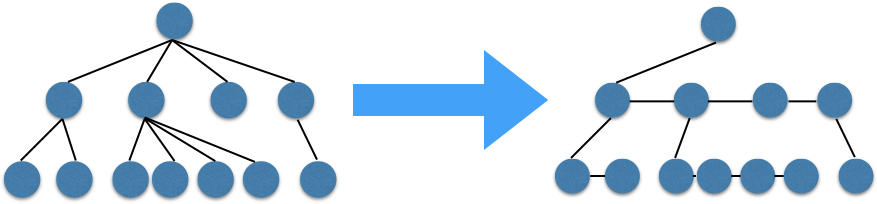
\includegraphics[width=7cm]{asset/lcrs.png}
\end{center}
\end{frame}

\begin{frame}[fragile]
\frametitle{DP pada Tree: Left-Child Right-Sibling (lanj.)}
\begin{lstlisting}
int g(int u, bool root, int take) {
  if (take == 0 || u == NULL) {
    return 0;
  }
  if (computed[u][root][take]) {
    return memo[u][root][take];
  }
  memo[u][root][take] = true;
  res = INT_MIN;
  for (int i = 0; i <= take; ++i) {
    res = max(res, g(child(u), true, i) + g(sibling(u), root, take - i));
    if (i < take) {
      // Mengambil node u, sehingga node child(u) tidak dapat diambil.
      res = max(res, w[u]
                   + g(child(u), false, i)
                   + g(sibling(u), root, take - i - 1));
    }
  }
  return memo[u][root][take] = res;
}
\end{lstlisting}
\end{frame}

\begin{frame}[fragile]
\frametitle{DP pada Tree: Mengubah menjadi Left-Child Right-Sibling}
\begin{lstlisting}
void dfs(int u, int parent) {
  child[u] = NULL;
  sibling[u] = NULL;
  int last_child = NULL;
  for (int x : adj[u]) { 
    if (x == parent) {
      continue;
    }
    if (child[u] == NULL) {
      child[u] = x;
    }
    if (last_child != NULL) {
      sibling[last_child] = x;
    }
    dfs(x, u);
    last_child = x;
  }
}
\end{lstlisting}
\end{frame}

\begin{frame}
\frametitle{Kompleksitas Solusi}
\begin{itemize}
  \item Jawaban yang diinginkan adalah $g(R, false, K)$ dengan $R$ adalah \froot \ftree.
  \item Banyaknya kemungkinan parameter pada fungsi $g$ di slide sebelumnya adalah $O(N \times K)$ dengan $N$ adalah banyaknya \fnode.
  \item Setiap fungsi $g$ mencoba seluruh pembagian $take$ ke dua \fnode, sehingga membutuhkan waktu $O(K)$.
  \item Sehingga, total kompleksitas dari solusi \fdp ini adalah $O(N \times K^2)$.
\end{itemize}
\end{frame}

\end{document}
